%%
% Copyright (c) 2017 - 2021, Pascal Wagler;
% Copyright (c) 2014 - 2021, John MacFarlane
%
% All rights reserved.
%
% Redistribution and use in source and binary forms, with or without
% modification, are permitted provided that the following conditions
% are met:
%
% - Redistributions of source code must retain the above copyright
% notice, this list of conditions and the following disclaimer.
%
% - Redistributions in binary form must reproduce the above copyright
% notice, this list of conditions and the following disclaimer in the
% documentation and/or other materials provided with the distribution.
%
% - Neither the name of John MacFarlane nor the names of other
% contributors may be used to endorse or promote products derived
% from this software without specific prior written permission.
%
% THIS SOFTWARE IS PROVIDED BY THE COPYRIGHT HOLDERS AND CONTRIBUTORS
% "AS IS" AND ANY EXPRESS OR IMPLIED WARRANTIES, INCLUDING, BUT NOT
% LIMITED TO, THE IMPLIED WARRANTIES OF MERCHANTABILITY AND FITNESS
% FOR A PARTICULAR PURPOSE ARE DISCLAIMED. IN NO EVENT SHALL THE
% COPYRIGHT OWNER OR CONTRIBUTORS BE LIABLE FOR ANY DIRECT, INDIRECT,
% INCIDENTAL, SPECIAL, EXEMPLARY, OR CONSEQUENTIAL DAMAGES (INCLUDING,
% BUT NOT LIMITED TO, PROCUREMENT OF SUBSTITUTE GOODS OR SERVICES;
% LOSS OF USE, DATA, OR PROFITS; OR BUSINESS INTERRUPTION) HOWEVER
% CAUSED AND ON ANY THEORY OF LIABILITY, WHETHER IN CONTRACT, STRICT
% LIABILITY, OR TORT (INCLUDING NEGLIGENCE OR OTHERWISE) ARISING IN
% ANY WAY OUT OF THE USE OF THIS SOFTWARE, EVEN IF ADVISED OF THE
% POSSIBILITY OF SUCH DAMAGE.
%%

%%
% This is the Eisvogel pandoc LaTeX template.
%
% For usage information and examples visit the official GitHub page:
% https://github.com/Wandmalfarbe/pandoc-latex-template
%%

% Options for packages loaded elsewhere
\PassOptionsToPackage{unicode}{hyperref}
\PassOptionsToPackage{hyphens}{url}
\PassOptionsToPackage{dvipsnames,svgnames*,x11names*,table}{xcolor}
%
\documentclass[
  french,
  paper=a4,
  ,captions=tableheading
]{scrartcl}
\usepackage{amsmath,amssymb}
\usepackage{lmodern}
\usepackage{setspace}
\setstretch{1.2}
\usepackage{ifxetex,ifluatex}
\ifnum 0\ifxetex 1\fi\ifluatex 1\fi=0 % if pdftex
  \usepackage[T1]{fontenc}
  \usepackage[utf8]{inputenc}
  \usepackage{textcomp} % provide euro and other symbols
\else % if luatex or xetex
  \usepackage{unicode-math}
  \defaultfontfeatures{Scale=MatchLowercase}
  \defaultfontfeatures[\rmfamily]{Ligatures=TeX,Scale=1}
\fi
% Use upquote if available, for straight quotes in verbatim environments
\IfFileExists{upquote.sty}{\usepackage{upquote}}{}
\IfFileExists{microtype.sty}{% use microtype if available
  \usepackage[]{microtype}
  \UseMicrotypeSet[protrusion]{basicmath} % disable protrusion for tt fonts
}{}
\makeatletter
\@ifundefined{KOMAClassName}{% if non-KOMA class
  \IfFileExists{parskip.sty}{%
    \usepackage{parskip}
  }{% else
    \setlength{\parindent}{0pt}
    \setlength{\parskip}{6pt plus 2pt minus 1pt}}
}{% if KOMA class
  \KOMAoptions{parskip=half}}
\makeatother
\usepackage{xcolor}
\definecolor{default-linkcolor}{HTML}{A50000}
\definecolor{default-filecolor}{HTML}{A50000}
\definecolor{default-citecolor}{HTML}{4077C0}
\definecolor{default-urlcolor}{HTML}{4077C0}
\IfFileExists{xurl.sty}{\usepackage{xurl}}{} % add URL line breaks if available
\IfFileExists{bookmark.sty}{\usepackage{bookmark}}{\usepackage{hyperref}}
\hypersetup{
  pdftitle={Challenge-response authentication protocole},
  pdfauthor={Simon Meier},
  pdflang={fr},
  pdfsubject={Sécurité},
  pdfkeywords={Security, CHAP},
  hidelinks,
  breaklinks=true,
  pdfcreator={LaTeX via pandoc with the Eisvogel template}}
\urlstyle{same} % disable monospaced font for URLs
\usepackage[bmargin=2.5cm, tmargin=2.5cm, lmargin=3.75cm, rmargin=2.25cm,includehead=true,includefoot=true,centering]{geometry}
\usepackage[export]{adjustbox}
\usepackage{graphicx}
\usepackage{longtable,booktabs,array}
\usepackage{calc} % for calculating minipage widths
% Correct order of tables after \paragraph or \subparagraph
\usepackage{etoolbox}
\makeatletter
\patchcmd\longtable{\par}{\if@noskipsec\mbox{}\fi\par}{}{}
\makeatother
% Allow footnotes in longtable head/foot
\IfFileExists{footnotehyper.sty}{\usepackage{footnotehyper}}{\usepackage{footnote}}
\makesavenoteenv{longtable}
% add backlinks to footnote references, cf. https://tex.stackexchange.com/questions/302266/make-footnote-clickable-both-ways
\usepackage{footnotebackref}
\usepackage{graphicx}
\makeatletter
\def\maxwidth{\ifdim\Gin@nat@width>\linewidth\linewidth\else\Gin@nat@width\fi}
\def\maxheight{\ifdim\Gin@nat@height>\textheight\textheight\else\Gin@nat@height\fi}
\makeatother
% Scale images if necessary, so that they will not overflow the page
% margins by default, and it is still possible to overwrite the defaults
% using explicit options in \includegraphics[width, height, ...]{}
\setkeys{Gin}{width=\maxwidth,height=\maxheight,keepaspectratio}
% Set default figure placement to htbp
\makeatletter
\def\fps@figure{htbp}
\makeatother
\setlength{\emergencystretch}{3em} % prevent overfull lines
\providecommand{\tightlist}{%
  \setlength{\itemsep}{0pt}\setlength{\parskip}{0pt}}
\setcounter{secnumdepth}{5}

% Make use of float-package and set default placement for figures to H.
% The option H means 'PUT IT HERE' (as  opposed to the standard h option which means 'You may put it here if you like').
\usepackage{float}
\floatplacement{figure}{H}

\ifxetex
    % See issue https://github.com/reutenauer/polyglossia/issues/127
  \renewcommand*\familydefault{\sfdefault}
    % Load polyglossia as late as possible: uses bidi with RTL langages (e.g. Hebrew, Arabic)
  \usepackage{polyglossia}
  \setmainlanguage[]{french}
\else
  \usepackage[main=french]{babel}
% get rid of language-specific shorthands (see #6817):
\let\LanguageShortHands\languageshorthands
\def\languageshorthands#1{}
\fi
\ifluatex
  \usepackage{selnolig}  % disable illegal ligatures
\fi

\title{Challenge-response authentication protocole}
\usepackage{etoolbox}
\makeatletter
\providecommand{\subtitle}[1]{% add subtitle to \maketitle
  \apptocmd{\@title}{\par {\large #1 \par}}{}{}
}
\makeatother
\subtitle{Sécurité}
\author{Simon Meier}
\date{\today}



%%
%% added
%%

%
% language specification
%
% If no language is specified, use English as the default main document language.
%


\usepackage[pages=all]{background}

%
% for the background color of the title page
%
\usepackage{pagecolor}
\usepackage{afterpage}
\usepackage{tikz}
\usepackage[bmargin=2.5cm, tmargin=2.5cm, lmargin=3.75cm, rmargin=2.25cm,includehead=true,includefoot=true,centering]{geometry}


%
% break urls
%
\PassOptionsToPackage{hyphens}{url}

%
% When using babel or polyglossia with biblatex, loading csquotes is recommended
% to ensure that quoted texts are typeset according to the rules of your main language.
%
\usepackage{csquotes}

%
% captions
%
\definecolor{caption-color}{HTML}{777777}
\usepackage[font={stretch=1.2}, textfont={color=caption-color}, position=top, skip=4mm, labelfont=bf, singlelinecheck=false, justification=raggedright]{caption}
\setcapindent{0em}

%
% blockquote
%
\definecolor{blockquote-border}{RGB}{221,221,221}
\definecolor{blockquote-text}{RGB}{119,119,119}
\usepackage{mdframed}
\newmdenv[rightline=false,bottomline=false,topline=false,linewidth=3pt,linecolor=blockquote-border,skipabove=\parskip]{customblockquote}
\renewenvironment{quote}{\begin{customblockquote}\list{}{\rightmargin=0em\leftmargin=0em}%
\item\relax\color{blockquote-text}\ignorespaces}{\unskip\unskip\endlist\end{customblockquote}}

%
% Source Sans Pro as the de­fault font fam­ily
% Source Code Pro for monospace text
%
% 'default' option sets the default
% font family to Source Sans Pro, not \sfdefault.
%
\ifnum 0\ifxetex 1\fi\ifluatex 1\fi=0 % if pdftex
    \usepackage[default]{sourcesanspro}
  \usepackage{sourcecodepro}
  \else % if not pdftex
    \usepackage[default]{sourcesanspro}
  \usepackage{sourcecodepro}

  % XeLaTeX specific adjustments for straight quotes: https://tex.stackexchange.com/a/354887
  % This issue is already fixed (see https://github.com/silkeh/latex-sourcecodepro/pull/5) but the
  % fix is still unreleased.
  % TODO: Remove this workaround when the new version of sourcecodepro is released on CTAN.
  \ifxetex
    \makeatletter
    \defaultfontfeatures[\ttfamily]
      { Numbers   = \sourcecodepro@figurestyle,
        Scale     = \SourceCodePro@scale,
        Extension = .otf }
    \setmonofont
      [ UprightFont    = *-\sourcecodepro@regstyle,
        ItalicFont     = *-\sourcecodepro@regstyle It,
        BoldFont       = *-\sourcecodepro@boldstyle,
        BoldItalicFont = *-\sourcecodepro@boldstyle It ]
      {SourceCodePro}
    \makeatother
  \fi
  \fi

%
% heading color
%
\definecolor{heading-color}{RGB}{40,40,40}
\addtokomafont{section}{\color{heading-color}}
% When using the classes report, scrreprt, book,
% scrbook or memoir, uncomment the following line.
%\addtokomafont{chapter}{\color{heading-color}}

%
% variables for title, author and date
%
\usepackage{titling}
\title{Challenge-response authentication protocole}
\author{Simon Meier}
\date{\today}

%
% tables
%

\definecolor{table-row-color}{HTML}{F5F5F5}
\definecolor{table-rule-color}{HTML}{999999}

%\arrayrulecolor{black!40}
\arrayrulecolor{table-rule-color}     % color of \toprule, \midrule, \bottomrule
\setlength\heavyrulewidth{0.3ex}      % thickness of \toprule, \bottomrule
\renewcommand{\arraystretch}{1.3}     % spacing (padding)


%
% remove paragraph indention
%
\setlength{\parindent}{0pt}
\setlength{\parskip}{6pt plus 2pt minus 1pt}
\setlength{\emergencystretch}{3em}  % prevent overfull lines

%
%
% Listings
%
%


%
% header and footer
%
\usepackage{fancyhdr}

\fancypagestyle{eisvogel-header-footer}{
  \fancyhead{}
  \fancyfoot{}
  \lhead[\today]{Challenge-response authentication protocole}
  \chead[]{}
  \rhead[Challenge-response authentication protocole]{\today}
  \lfoot[\thepage]{Simon Meier}
  \cfoot[]{}
  \rfoot[Simon Meier]{\thepage}
  \renewcommand{\headrulewidth}{0.4pt}
  \renewcommand{\footrulewidth}{0.4pt}
}
\pagestyle{eisvogel-header-footer}
\backgroundsetup{
scale=1,
color=black,
opacity=0.2,
angle=0,
contents={%
  \includegraphics[width=\paperwidth,height=\paperheight]{backgrounds/background\_page.png}
  }%
}

%%
%% end added
%%

\begin{document}

%%
%% begin titlepage
%%
\begin{titlepage}
\newgeometry{top=2cm, right=4cm, bottom=3cm, left=4cm}
\definecolor{titlepage-color}{HTML}{ffd7d4}
\newpagecolor{titlepage-color}\afterpage{\restorepagecolor}
\tikz[remember picture,overlay] \node[inner sep=0pt] at (current page.center){\includegraphics[width=\paperwidth,height=\paperheight]{backgrounds/background\_frontpage.png}};
\newcommand{\colorRule}[3][black]{\textcolor[HTML]{#1}{\rule{#2}{#3}}}
\begin{flushleft}
\noindent
\\[-1em]
\color[HTML]{242424}
\makebox[0pt][l]{\colorRule[360049]{1.3\textwidth}{4pt}}
\par
\noindent

% The titlepage with a background image has other text spacing and text size
\noindent

\includegraphics[width=105mm, left]{images/arc-logo.png}

{
  \setstretch{2}
  \vfill
  \vskip -8em
  \noindent {\Huge \textbf{\textsf{Challenge-response authentication
protocole}}}
    \vskip 1em
  {\huge \textsf{Sécurité}}
    \vskip 2em
  \noindent {\Large \textsf{Étudiant: Simon Meier} \vskip 0.3em \textsf{Professeur: Marc Schaefer} \vskip 0.3em \textsf{\today}}
  \vfill
}


\end{flushleft}
\end{titlepage}
\restoregeometry

%%
%% end titlepage
%%


\tableofcontents

\begin{center}\rule{0.5\linewidth}{0.5pt}\end{center}

\textbf{Titre:} Exercice à rendre: challenge-response

\textbf{Etudiant:} Simon Meier

\textbf{Professeur:} Marc Schaefer

\begin{center}\rule{0.5\linewidth}{0.5pt}\end{center}

\hypertarget{arborescence-du-projet}{%
\section{Arborescence du projet}\label{arborescence-du-projet}}

\begin{verbatim}
exercice4
|   readme.md
|   requirements.txt
|---.venv
|---__pycach__
|---images
|---backgrounds
|---challenge_response_authentication
       client.py
       cryptool.py
       main.py
       server.py
\end{verbatim}

\newpage

\hypertarget{challenge-response-authentication-protocole}{%
\section{Challenge-response authentication
protocole}\label{challenge-response-authentication-protocole}}

\hypertarget{consigne}{%
\subsection{Consigne}\label{consigne}}

\begin{quote}
Voir
\url{https://en.wikipedia.org/wiki/Challenge\%E2\%80\%93response_authentication}
Tenir compte des recommandations
\href{02_Authentification/autres/nma-hash-crypt-PRNG-recommandations.pdf}{hash,
crypto, PRNG}. PS: nous avons déjà vu un tel protocole
challenge-response dans le CHAP des slides ainsi que pour
l'authentification d'un téléphone IP à Asterisk en R+A 2e année.
\end{quote}

\textbf{Délai: fin de la semaine des présentations.}


\hypertarget{exercice-uxe0-rendre-challenge-response}{%
\subsubsection{4. Exercice à rendre:
challenge-response}\label{exercice-uxe0-rendre-challenge-response}}

Dans le langage de votre choix et par groupe de deux, implémentez un
client et un serveur d'authentification basé sur un challenge-response.

Indications (répondre aux questions en commentaire dans le code)

\hypertarget{questions}{%
\subsubsection{Questions}\label{questions}}



\begin{itemize}
\tightlist
\item
  quel hachage cryptographique utilisez-vous et pourquoi?

  \begin{itemize}
  \tightlist
  \item
    J'utilise MD5(pour Message Digest 5). C'est une fonction de hachage
    cryptographique qui permet d'obtenir l'empreinte numérique d'une
    variable, par exemple une chaîne de caractère. Il est aujourd'hui
    dépassé et absolument impropre à toute utilisation en cryptographie
    ou en sécurité. Le seul intérêt ici est qu'il convient bien à
    l'exercice d'implémentation du challenge-response protocole.
  \end{itemize}
\item
  quelles précautions pour le générateur aléatoire?

  \begin{itemize}
  \tightlist
  \item
    utilisation du module `secrets' et de la fonction
    \texttt{tocken\_hex()} pour générer une chaîne de caractère
    aléatoire. La différence comparé au module random de base est que le module random ne fournit pas des nombres suffisamment aléatoire, comme elle suit une distribution uniforme et que si elle est basée sur le temps, elle est assez facile à prédire.  Une attaque en brute force est alors suffisante aujourd'hui pour mettre en péril ce genre de génération aléatoire. C'est pourquoi il est nécessaire d'utiliser des fonctions plus élaborées, qui prennent en paramètre des sources de l'OS pour produire des nombres aléatoires. En revanche, l'on pourrait imaginer aujourd'hui des systèmes de réseaux de neurones qui apprendraient les valeurs de ces sources par catégories d'OS et ainsi prédire la distribution de ces valeurs. Tout système à ces limites, malgré tout c'est toujours mieux que d'utiliser le module random de base.
  \end{itemize}
\item
  quelles précautions pour la construction garantissant l'unicité du
  nonce?

  \begin{itemize}
  \tightlist
  \item
    il ne doit pas se répéter; ici, une boucle vérifie si le nonce
    existe déjà dans une liste. Cette opération est faite lors de
    l'utilisation de la fonction \texttt{createNonce()}.
  \end{itemize}
\item
  quelles précautions pour la durée de validité du nonce?

  \begin{itemize}
  \tightlist
  \item
    le nonce est unique et généré à chaque fois que le challenge est
    envoyé.
  \end{itemize}
\item
  la partie réseau n'est pas nécessaire: des appels de fonctions simples
  sont autorisés.
\end{itemize}

\hypertarget{utilisation-du-programme}{%
\subsection{Utilisation du programme}\label{utilisation-du-programme}}

\begin{enumerate}
\def\labelenumi{\arabic{enumi}.}
\item
  Activez le \texttt{.venv} que vous avez configurer avec le 1er
  \texttt{readme} du projet:
\begin{verbatim}
source .venv/Scripts/activate
\end{verbatim}
\item
  Naviguez jusqu'à être dans le dossier:
  \texttt{/exercice4/challenge\_response\_authentication}
\item
  Lancer le programme:
\begin{verbatim}
python .\main.py
\end{verbatim}
\end{enumerate}

\hypertarget{exemple-de-sortie-du-programme}{%
\subsubsection{Exemple de sortie du
programme}\label{exemple-de-sortie-du-programme}}

\begin{longtable}[]{@{}c@{}}
\toprule
Output\tabularnewline
\midrule
\endhead
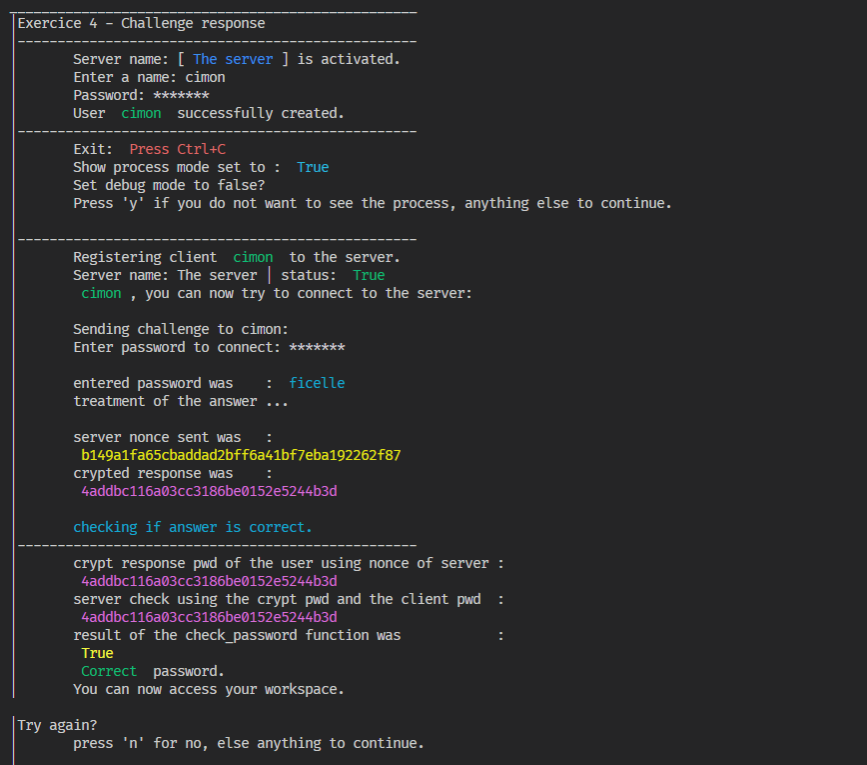
\includegraphics[width=105mm]{images/i1.png}\tabularnewline
\bottomrule
\end{longtable}

\hypertarget{protocole-choisi-chap}{%
\subsubsection{Protocole choisi: CHAP}\label{protocole-choisi-chap}}

Le protocole CHAP (Challenge Handshake Authentication Protocol) est un
protocole d'authentification point à point (PPP) développé par l'IETF
(Internet Engineering Task Force). Il est utilisé au démarrage initial
du lien. En outre, il effectue des vérifications périodiques pour
vérifier si le routeur communique toujours avec le même hôte.

\begin{itemize}
\tightlist
\item
  CHAP:

  \begin{itemize}
  \tightlist
  \item
    utilise le protocole d'établissement de liaison à 3 voies (pas comme
    TCP). Tout d'abord, l'authentificateur envoie un paquet de défi au
    pair, puis le pair répond avec une valeur en utilisant sa fonction
    de hachage à sens unique. L'authentificateur fait alors correspondre
    la valeur reçue avec sa propre valeur de hachage calculée. Si les
    valeurs correspondent, l'authentification est confirmée, sinon
    invitation à ce que l'utilisateur réessaie.
  \item
    utilise une fonction de hachage unidirectionnelle appelée MD5.
  \item
    s'authentifie également périodiquement pour vérifier si la
    communication a lieu avec le même appareil ou non.
  \item
    offre plus de sécurité que PAP (Password Authentication Procedure)
    car la valeur utilisée (découverte par la fonction de hachage) est
    modifiée de manière variable.
  \item
    nécessite de connaître le texte en clair du secret car il n'est
    jamais envoyé sur le réseau.
  \end{itemize}
\end{itemize}

\end{document}
